\chapter{Introduzione}

\section{Malware e tipologie}
Nell'ambito della sicurezza informatica, un malware è definito come un software che attua comportamenti malevoli contrari alla volontà dell'utente finale con lo scopo di modificare il normale funzionamento di un sistema, a illegittimo vantaggio del suo autore e ai danni dell'utente \cite{malwarebytes_malware_definition}.

Possono essere di varie tipologie, o unioni di alcune di esse:
\begin{itemize}
    \item \textbf{Adware}: progettati per presentare messaggi pubblicitari e guadagnare da essi
    \item \textbf{Spyware}: hanno lo scopo di osservare le azioni dell'utente senza il suo permesso per poi riportare il tutto all'autore
    \item \textbf{Virus}: vanno ad alterare altri programmi agganciandoci del proprio codice
    \item \textbf{Worm}: alterano altri computer in una stessa rete, provocando danni
    \item \textbf{Trojan}: ingannano l'utente presentandosi come un software utile, che quindi l'utente va ad installare volontariamente, non sapendo cosa si cela realmente al contrario di ciò che gli è stato promesso
    \item \textbf{Ransomware}: guadagnano sul malcapitato criptando tutti i propri file importanti, chiedendo poi un riscatto in criptovalute per lo sblocco - qui si fa leva sull'importanza e l'assenza di backup di dati importanti e sul proprio valore sia economico che morale (a seconda che si tratti di un'azienda o di un utente domestico)
    \item \textbf{Rootkit}: sfruttano vulnerabilità nel sistema target per ottenere privilegi da amministratore
\end{itemize}
Com'è normale pensare, non esistono solo questi tipi, ma sono solo alcuni dei più famosi.

Infine, per maggiore comprensione delle seguenti illustrazioni, è bene spiegare altri pochi termini:
\begin{itemize}
    \item Una \textbf{vulnerabilità} è rappresentata da una criticità in un componente di un sistema informatico, come l'assenza di misure di sicurezza o la propria compromissione
    \item Un \textbf{exploit} invece è un software o un insieme di comandi che vanno a sfruttare la vulnerabilità a proprio vantaggio, al fine di provocare un comportamento altrimenti inaspettato
    \item Un tipo particolare di exploit chiamato \textbf{zero-day} va a sfruttare falle non note prima dell'attacco, provocando così potenzialmente molti più danni, non essendo ancora disponibile una patch del software vulnerabile
    \item Per \textbf{IoC} si intende un Indicator of Compromise, indicatore usato per identificare indirizzi IP o nomi di dominio di C\&C, hash di file, firme di antivirus, o altro, che faccia ricondurre con alta probabilità a una specifica intrusione
\end{itemize}

\subsection{MITRE ATT\&CK}
\label{chap:mitre_attack}

\begin{figure}[htbp]
    \centering
    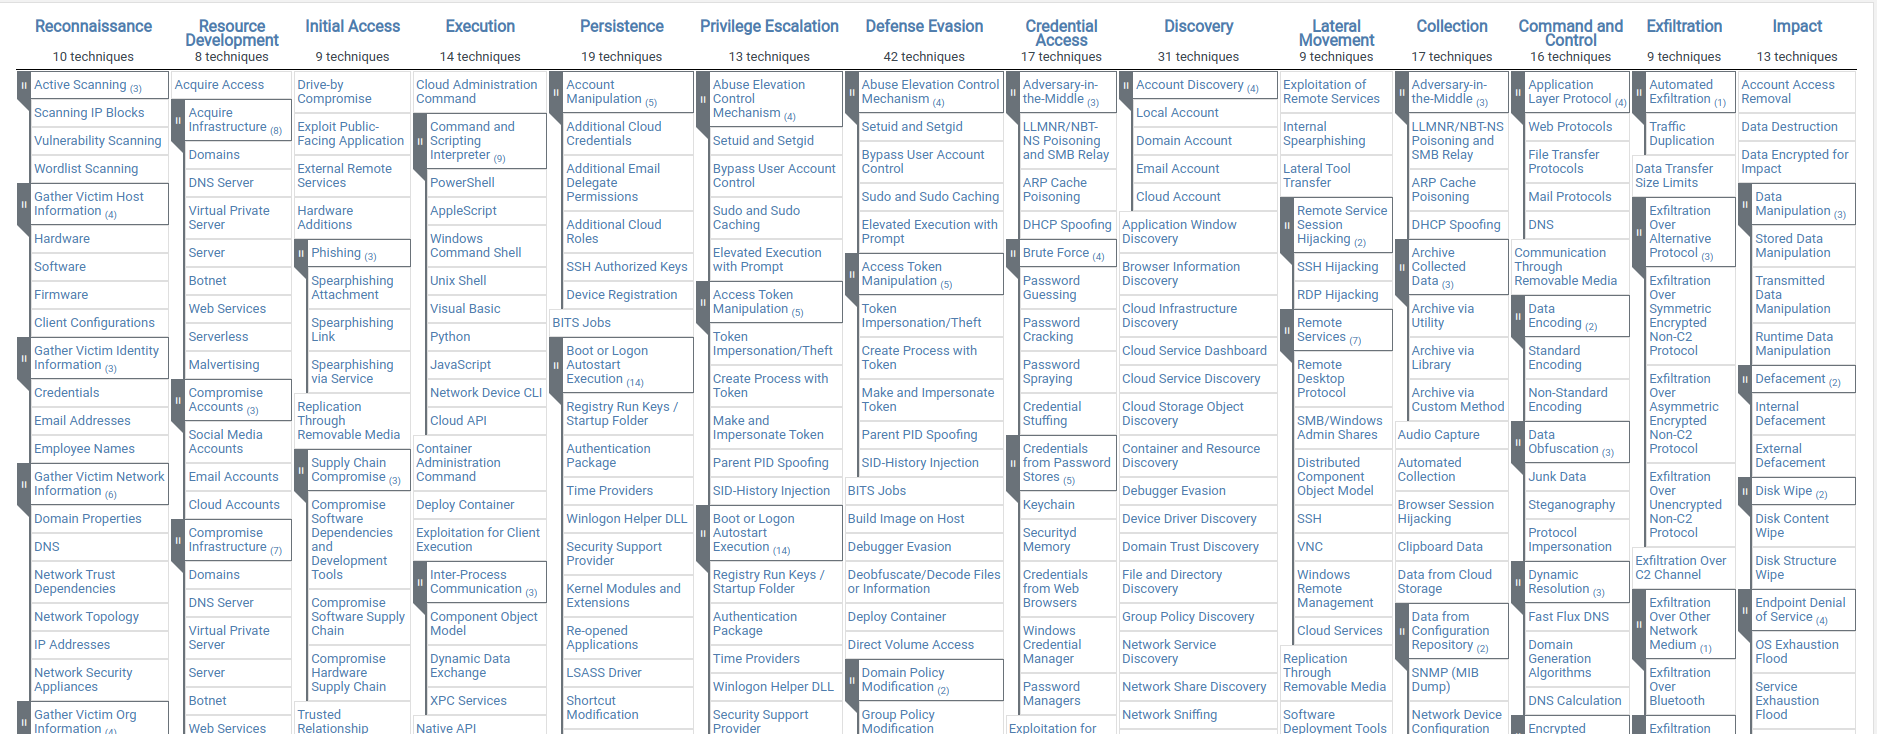
\includegraphics[width=\textwidth]{assets/mitre_attack_matrix.png}
    \caption{MITRE ATT\&CK Matrix for Enterprise}
    \label{fig:mitre_attack_matrix}
\end{figure}

Per identificare più precisamente le tipologie di malware che stiamo trattando, si va ad usare il \emph{MITRE ATT\&CK® Framework} (Adversarial Tactics, Techniques, and Common Knowledge)
\footnote{Pagina ufficiale MITRE ATT\&CK: \url{https://attack.mitre.org/}}.

Si tratta di una base di conoscenza sviluppata da MITRE Corporation, che include tattiche e adversary techniques, basata osservando gli avvenimenti nel mondo reale. Nato nel 2013 con lo scopo di descrivere le più comuni tattiche, tecniche e procedure \emph{(TTP)} usate nei sistemi Windows enterprise, ad uso interno MITRE, è poi diventato lo standard de-facto per la descrizione di tali aspetti di un attacco
\cite{mitre_attack_framework_introduction}, per far fronte all'assenza di una tassonomia comune per la descrizione dei TTP.

Si focalizza sulle interazioni che il malware ha col sistema target, e raggruppa questi comportamenti in tattiche per fornire più contesto sulla tecnica utilizzata.
\begin{itemize}
    \item Le \textbf{tattiche} sono il \emph{perché} di una tecnica, indicando l'obiettivo che si intende perseguire, e servono da contenitore per le varie tecniche; nello standard iniziano per \texttt{TA} (es: \texttt{TA0043} - Reconnaissance - Ricognizione, l'avversario va ad ottenere informazioni sul sistema per capire come muoversi)
    \item Le \textbf{tecniche} invece sono il \emph{come} di una specifica azione, e potrebbero far dedurre anche il \emph{cosa} un avversario ottiene come risultato della sua azione - particolarmente utile nella tattica TA0007 Discovery, dove si cerca di studiare la composizione del sistema target. \\
    Una tecnica è spesso composta da sotto-tecniche per essere ancora più specifici.
    Ad esempio, la tecnica \texttt{T1595.002} Vulnerability Scanning (dove si va capendo i software disponibili sul sistema target e la loro versione, con il possibile scopo di verificare se si allinea a una specifica versione vulnerabile di cui l'avversario già dispone di un exploit) è sotto-tecnica di \texttt{T1595} Active Scanning, e fa parte della tattica \texttt{TA0043} Reconnaissance vista al punto precedente.
\end{itemize}

Nella matrice in figura \ref{fig:mitre_attack_matrix}, le tattiche sono le colonne e le tecniche sono le celle, possibilmente composte da sotto-tecniche.

Viene usato anche per l'integrazione con la Cyber Threat Intelligence, che vedremo nella sezione \ref{chap:cyber_threat_intelligence}, punto focale anche degli strumenti realizzati nel progetto.

\section{Cyber Kill Chain}
Partendo dalle tattiche appena viste, possiamo costruire ciò che è noto col nome di \emph{Cyber Kill Chain}.
Si tratta di un modello simile al MITRE ATT\&CK framework (sez. \ref{chap:mitre_attack}), ma segue un diverso approccio. Qui infatti si vanno a ripercorrere le 7 tipiche fasi cronologiche di un attacco ad un sistema informatico, fornendo una panoramica più ad alto livello.

\begin{figure}[h]
    \centering
    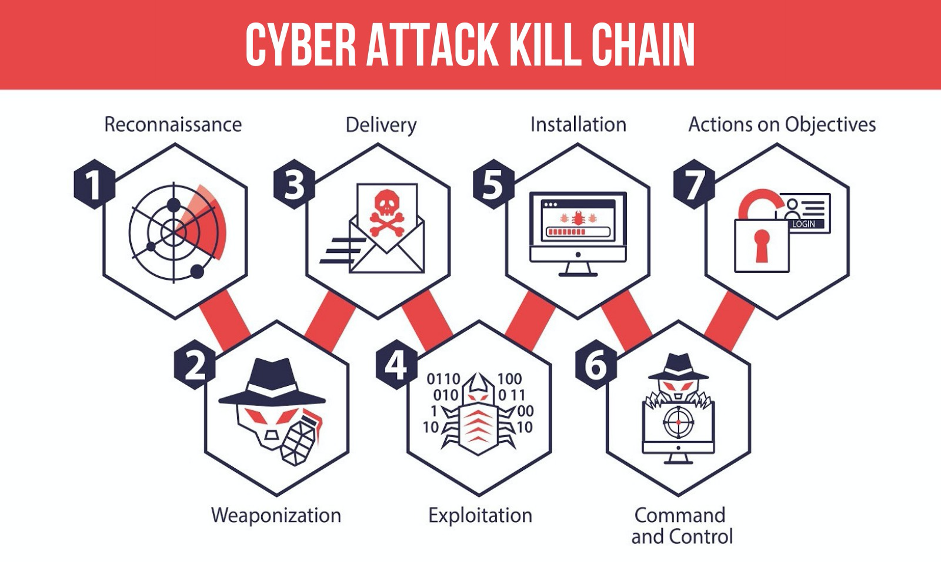
\includegraphics[width=0.6\textwidth]{assets/cyber_kill_chain.png}
    \caption{(crediti immagine: "Fondazione F3RM1")}
    \label{fig:cyber_kill_chain}
\end{figure}

Si compone delle seguenti fasi \cite{cyber_kill_chain_360}, portando un esempio tipico:
\begin{enumerate}
    \item \textbf{Ricognizione}: identificazione dei punti di accesso a un sistema e sue vulnerabilità, derivabili tramite analisi attiva (uso di strumenti come \emph{nmap} in maniera più o meno aggressiva) o passiva, leggendo informazioni già da fonti note (come \emph{Shodan.io} partendo da un indirizzo IP): ad esempio, possiamo notare come siano presenti ed esposti servizi con versioni obsolete / vulnerabili
    
    \item \textbf{Armamento}: creazione del vero e proprio malware da utilizzare nell'attacco, nell'intento di sfruttare la vulnerabilità individuata - ad esempio creiamo un pacchetto IP con scapy

    \item \textbf{Consegna}: il payload creato deve essere consegnato alla vittima in qualche modo, come una mail di phishing o un form di una pagina del sito web - quindi inviamo il pacchetto al server al suo indirizzo IP pubblico

    \item \textbf{Exploit}: nella realtà dei fatti, si sta sfruttando una vulnerabilità individuata - nel nostro caso reale, potremmo aver scatenato una RCE (Remote Code Execution) o altre tecniche

    \item \textbf{Installazione}: dopo la riuscita dell'exploit, si scarica e avvia il payload malevolo, cercando di bypassare strategie esistenti di rilevazione, usando metodologie come obfuscation - nell'esempio, possiamo installare una reverse shell ad avvio automatico in file come `~/.bashrc` o `~/.profile`

    \item \textbf{Command and Control (C\&C)}: andiamo a instaurare un canale di comunicazione tra noi e la vittima, così da controllarlo da remoto - qui possono essere utili strumenti come Havoc C2.

    \item \textbf{Azioni sugli obiettivi}: eseguiamo le azioni più disparate, in base a ciò che vogliamo fare noi come attaccanti, come leggere un file contenenti informazioni sensibili o eseguire il dump del database
\end{enumerate}

\section{Tipi di sistemi di protezione}
Ora che abbiamo visto tutte queste minacce, viene spontaneo chiedersi come sia possibile proteggersi.

Il tipo più basilare di software per la protezione è l'\textbf{antivirus}. Questa tipologia di strumenti di protezione si va a concentrare sui singoli computer endpoint, e sfrutta modelli euristici per la rilevazione di vari tipi noti di malware, analizzando \emph{file su disco}.

Ben più potente è l'EDR, acronimo di \textbf{Endpoint Detection and Response}, che sfrutta l'\emph{analisi comportamentale} per rilevare e contrastare anche minacce sconosciute, basandosi sui loro comportamenti. Ad esempio, se vediamo che, dopo aver aperto un file scaricato da Internet, il processo del programma che ne permette la visualizzazione inizia a fare operazioni fuori dal normale funzionamento, come aprire una shell o modificare file o registri di sistema, sicuramente andrà terminato e riportato come incidente, che poi andrà gestito da chi di competenza.
La sostanziale differenza è il passaggio da semplice analisi su disco a una profonda analisi comportamentale, sfruttando strumenti forniti dal sistema operativo come Microsoft ETW \emph{(Event Tracing for Windows)} o eseguire l'hooking delle syscall manualmente - tecnica ben più complessa ed error-prone.

Infine, con un XDR (\textbf{eXtended Detection and Response}) andiamo ad allargare gli elementi sotto la protezione del software in questione, permettendo un'integrazione anche con reti, firewall, log di sicurezza e molto altro.
In questo modo, ha la potenza di aggregare e correlare eventi da più fonti, rilevando minacce sofisticate che verrebbero altrimenti ignorate.
Un esempio in questa categoria è \emph{SentinelOne XDR}.

\section{Cyber Threat Intelligence}
\label{chap:cyber_threat_intelligence}
L'area di Threat Intelligence si occupa di raccogliere tutta una serie di dati dai vari elementi,
per poi aggregarli e compiere analisi sulle informazioni ottenute, al fine di rilevare minacce anche sofisticate e prendere decisioni sulla sicurezza in maniera più veloce e consapevole.

La Threat Intelligence è un tassello estremamente importante nella sicurezza di un sistema informatico, soprattutto se unito al MITRE ATT\&CK framework: documentando i profili con cui l'avversario opera (come \texttt{APT29} - i profili sono insiemi di attività tipiche del modo di operare di alcuni gruppi nel panorama cyber), ma anche individuando la tecnica più efficacemente così da raggruppare tra loro più attacchi con caratteristiche comuni.
In questo modo, è possibile focalizzarsi maggiormente sulle tecniche che sono maggiormente usate in un dato profilo di attacco.

Esempi di come particolari avversari, delineati sotto un profilo, usano le proprie tecniche sono documentati nella pagina ATT\&CK corrispondente.
Studiandone la metodologia di attacco, è possibile replicarlo in fase di emulazione \emph{(Adversary Emulation)} per capire fino in fondo come difendersi da attacchi similari, e testare le proprie difese, nonché eseguire test di rilevazione.

Per questo e altri motivi, come vedremo, nella prima fase di analisi integreremo questo framework per la categorizzazione delle capabilities di un eseguibile.

\medskip

Un altro importante ruolo della Threat Intelligence, maggiormente vicino al progetto realizzato, è quello di analizzare i malware coinvolti negli attacchi noti o forniti da clienti qualora ne chiedessero l'analisi approfondita. Proprio a questo scopo, il proprio lavoro viene nettamente agevolato da strumenti di analisi automatica più estendibili possibile, così da avere fin da subito tutti i dati su cui lavorare.

\section{Contesto d'uso del progetto}
Una volta vista una panoramica superficiale di questo ambito della sicurezza informatica,
andiamo ad analizzare il contesto in cui si va ad inserire il progetto realizzato.

L'azienda ospitante offre, come suo core business, sistemi di EDR e XDR.
Questi sistemi usano programmi Agent installati nei vari endpoint, che sonde usate per analizzare il traffico di rete nei vari livelli ISO-OSI, nonché analisi sui dispositivi OT.

Soprattutto in riferimento all'Agent installato sugli endpoint, esso andrà a rilevare eseguibili con comportamenti anomali o sconosciuti e li andrà ad inviare al sistema di Threat Intelligence, che valuterà con una data confidence se siano o meno malevoli.
La capacità di eseguire detection di alta qualità è uno dei tratti distintivi tra le diverse soluzioni di sicurezza esistenti sul mercato e ha una diretta ripercussione sulla soddisfazione del cliente finale dell'azienda, oltre alla propria reputazione come brand.
Proprio in questo punto cruciale, viene l'esigenza dietro il progetto realizzato.

\subsection{Il problema da risolvere}
Lo scopo principale è la costruzione di un proprio sistema interno di analisi di malware automatizzata, eliminando le ultime dipendenze con servizi terzi quali VirusTotal, sia per un fattore economico che di flessibilità nei propri prodotti.

Un aspetto importante mantenuto chiaro per tutto il corso del progetto è proprio la flessibilità che deve essere garantita a questo nuovo strumento di essere esteso e maggiormente integrato nel corso della propria esistenza. Com'è intuibile infatti, il sistema qui creato verrà successivamente usato come base per la propria architettura di analisi malware automatizzata, che si andrà ad interfacciare con i vari prodotti.

\subsection{Interfacciamento con gli altri servizi}
\label{chap:intro_interface_with_other_services}

Il progetto si andrà ad integrare nella nuova architettura di sistema proprietaria dell'azienda ospitante.
Seppur è ancora in costruzione, per cui alcuni aspetti potrebbero variare tra il momento della scrittura e la loro effettiva realizzazione, ne viene delineato lo stato dell'arte.

Il punto di partenza è rappresentato dall'Agent, nominato poco fa e installato sui vari endpoint ove possibile, che raccoglie eseguibili sospetti e che reputa necessitino un'analisi più approfondita.
Siccome spesso si trova all'interno di una rete isolata, dove non è permessa la comunicazione con qualsiasi host Internet, può inviare gli eseguibili al COS. Più precisamente, inizialmente l'Agent non conosce ancora se siano già presenti analisi, così per questioni di efficienza invia solo il suo hash, inviando poi l'intero file solo in caso di esito negativo.

Il COS si occuperà di mantenere una coda di analisi, per non sovraccaricare il resto dei sistemi.
Invierà il file o l'hash ad FSL, che si pone come middleware per le API della Threat Intelligence.

Attualmente viene interrogata l'API di VirusTotal Enterprise per ottenere il maggior numero di informazioni, ma come abbiamo detto questa è la parte più critica a causa degli ingenti costi (fig. \ref{fig:fsl_general_arch_vt_success}).

In caso negativo, verrà invocato il progetto qui realizzato. Quindi, l'Agent invierà il file (non più l'hash) al COS, che lo inoltrerà alla nostra Sandbox, che si compone di una parte di analisi statica e di una dinamica (fig. \ref{fig:fsl_general_arch_sandbox_invoke}). Come vedremo, la fase di analisi statica avrà come trigger l'upload di un file su uno specifico bucket S3.

\section{Architettura generale della Sandbox}

Il sistema di analisi qui realizzato, chiamato per brevità anche \emph{Sandbox},
si compone di due parti, indipendenti l'una dall'altra al fine di mantenere una massima modularità.
Qui sono riportate come introduzione le due architetture in linea di massima, che verranno poi ben dettagliate nelle apposite sezioni di seguito.

Per quanto concerne l'aspetto statico, ci si avvarrà di Amazon Web Services per il funzionamento,
sfruttando principalmente i servizi di cloud storage S3 Bucket e di esecuzione Lambda, per minimizzare i costi e avere un sistema flessibile.
Una volta analizzato il file, la Threat Intelligence, mediante le sue API, riceverà gli stati di inizio e fine del processo, inclusi i risultati in un formato JSON concordato. Lo andrà a salvare e lo userà nelle future richieste con lo stesso hash (fig. \ref{fig:fsl_general_arch_sandbox_cached}).

Al contempo, l'aspetto dinamico si avvale di una già nota sandbox open-source quale Cuckoo Sandbox,
su cui è stato costruito il resto del sistema completo,
andando a installare il software, configurare il sistema a livello di firewall e SystemD Unit,
nonché creare nuovi moduli al fine di integrare tool nuovi, e un sistema di reporting che si basa su un client Python sviluppato appositamente per lo scopo.

\begin{figure}
    \centering
    \begin{subfigure}[b]{0.48\textwidth}
        \centering
        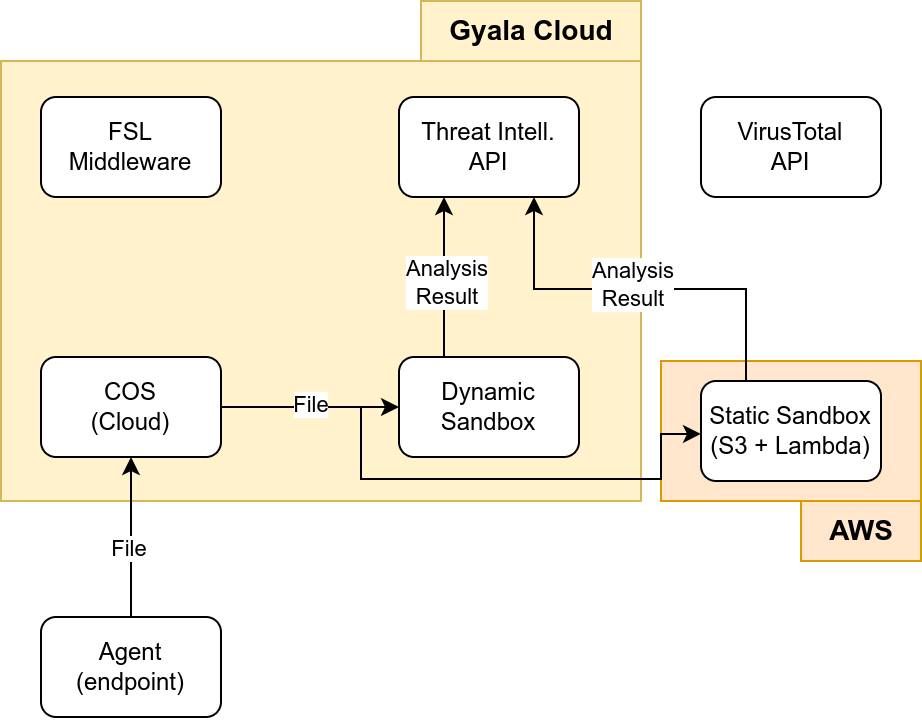
\includegraphics[width=\textwidth]{assets/fsl_general_arch_sandbox_invoke.png}
        \caption{Necessario invocare la sandbox}
        \label{fig:fsl_general_arch_sandbox_invoke}
    \end{subfigure}
    \begin{subfigure}[b]{0.48\textwidth}
        \centering
        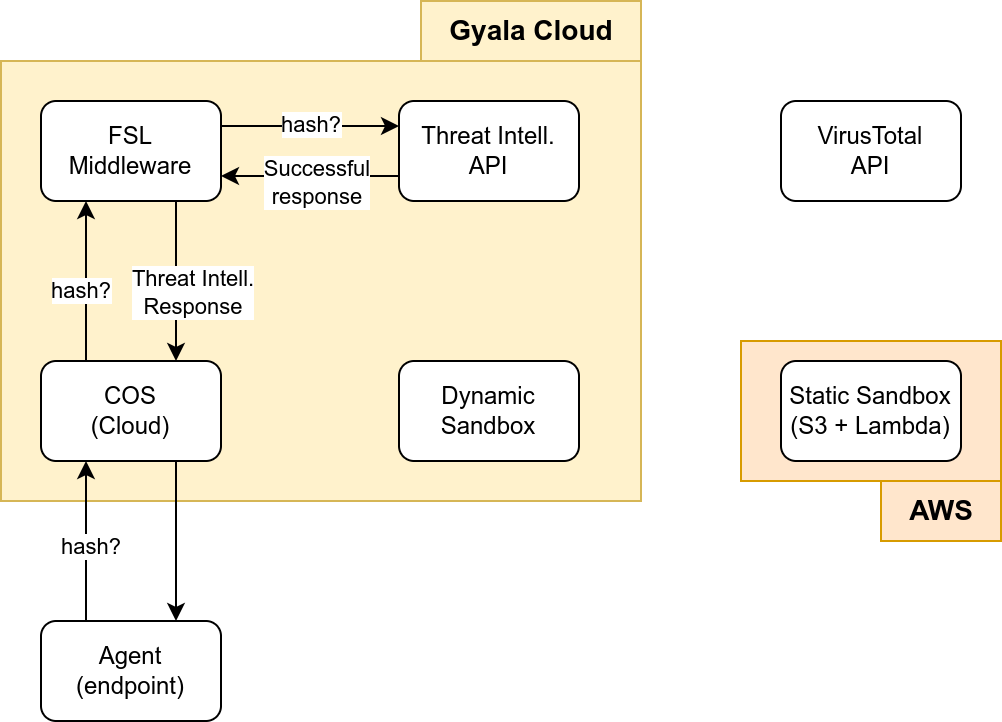
\includegraphics[width=\textwidth]{assets/fsl_general_arch_sandbox_cached.png}
        \caption{Risultati della Sandbox già in database}
        \label{fig:fsl_general_arch_sandbox_cached}
    \end{subfigure}
    \hfill
    \vspace{0.5cm}
    \hfill
    \begin{subfigure}[b]{0.48\textwidth}
        \centering
        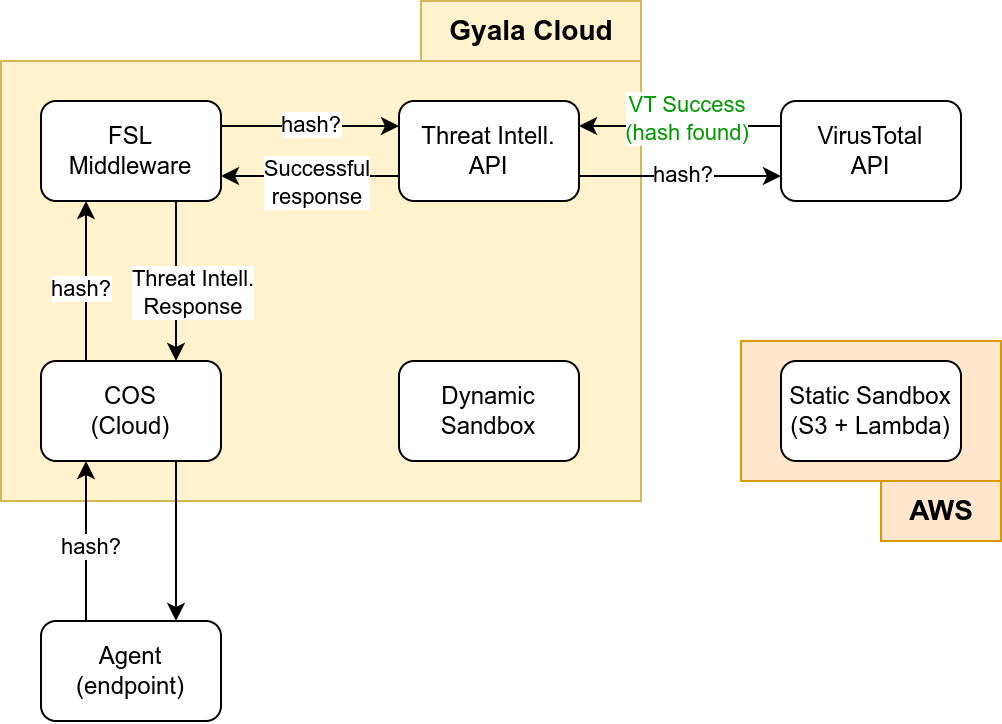
\includegraphics[width=\textwidth]{assets/fsl_general_arch_vt_success.png}
        \caption{Vecchio flusso prima della creazione della Sandbox}
        \label{fig:fsl_general_arch_vt_success}
    \end{subfigure}
    \caption{Schema generale di funzionamento dell'architettura nei vari casi}
    \label{fig:fsl_general_arch}
\end{figure}